\documentclass[a4paper]{tufte-handout}
\usepackage[utf8]{inputenc}

\newcommand{\workingDate}{\textsc{Nov $|$ 2018}}
\newcommand{\userName}{Ricardo Chávez Cáliz}
\newcommand{\institution}{CCM}
\newcommand{\R}{\mathbb{R}}
\newcommand{\Q}{\mathbb{Q}}
\newcommand{\N}{\mathbb{N}}
\newcommand{\Z}{\mathbb{Z}}
\renewcommand{\G}{\mathcal{G}}

\renewcommand{\P}{\mathbb{P}}

\usepackage{lab_notes}

\usepackage{hyperref}
\hypersetup{
    pdffitwindow=false,            % window fit to page
    pdfstartview={Fit},            % fits width of page to window
    pdftitle={Rigidity, curve complex and stochastic topology},     % document title
    pdfauthor={Ricardo Chávez Cáliz},         % author name
    pdfsubject={},                 % document topic(s)
    pdfnewwindow=true,             % links in new window
    colorlinks=true,               % coloured links, not boxed
    linkcolor=DarkScarletRed,      % colour of internal links
    citecolor=DarkChameleon,       % colour of links to bibliography
    filecolor=DarkPlum,            % colour of file links
    urlcolor=DarkSkyBlue           % colour of external links
}
\newtheorem{theorem}{Theorem}[section]
\newtheorem{defini}{Definition}[theorem]
\title{Rigidity phenomena in the curve complex in a stochastic perspective}
\date{Guanajuato - Nov 2018}

\begin{document}
\maketitle

%%%%%%%%%%%%%%%%%%%%%%%%%%%%%%%%%%%%%%%%%%%%%%%%%%%%%%%%

\begin{projects}
	\begin{description}
		\item [Advisor:] Noé Bárcenas Torres - Executive summary
	\end{description}
\end{projects}

%%%%%%%%%%%%%%%%%%%%%%%%%%%%%%%%%%%%%%%%%%%%%%%%%%%%%%%%
%\footnote{names and ideas changd to protect the innocent}
{\Large \noindent \textbf{Introduction}}

\justify
The study of surfaces in a strictly topological viewpoint has made us to forget significant information about them. A way to revert this is to attach a group to it, the \textbf{mapping class group} of the surface, it's denoted by $Mod(S)$ and encode the \textit{symmetries} of the surface. The \textbf{curve complex} of the surface, denoted by $C(S)$ appears naturally in the study of $Mod(S)$. It is a simplicial complex that encodes intersection patterns of simple closed curves in $S$. 

Many of the progress in understanding $Mod(S)$ has been possible by a well-known comparison among two very important classes of groups: arithmetic groups and mapping class groups. In this parallelism panorama arises the desire for an equivalent, until some extent, of the Margulis Superrigidity for mapping class groups. \footnote{The folkloric version of Mostow and Margulis superrigidity claims \textbf{that the only homomorphisms between lattices are the “obvious ones”}, in the $Mods(S)$ context this will mean that if we consider $X$ and $Y$, under suitable conditions, then every homomorphism $Mod(X) \to Mod(Y)$ will be induced by a manipulation of the underlying surfaces. }

We want to give an answer to the rather vague question: \textbf{\textit{How \textbf{common} is rigidity in the curve complex?}}

The idea of the thesis is to review properties of the curve complex of a surface so that a probabilistic model can be settled. Then we would like to use scientific computing to have a toy model to play with.

To extend the results of rigidity in simplicial maps there's an approach called \textit{rigid expansions} found  in [Armayona, 16]\cite{rigidExpJA} and [Hernández, 16]\cite{rigidExpJH}. This allows us to generate rigid sets from an initial one. We'll take particular interest in this point of view because of its combinatorial nature and therefore its compatibility with the stochastic background.

\noindent \hrulefill

%%%%%%%%%%%%%%%%%%%%%%%%%%%%%%%%%%%%%%%%%%%%%%%%%%%%%%%%
{\Large \noindent \textbf{The curve complex}}

The curve complex is build up using intersection pattern of curves in the surface. Among the adjectives that a curve can acquired we have the following:
\begin{itemize}
    \item A closed curve is called \textbf{essential} if it's not homotopic to a point, a puncture, or a boundary component.
    \item $\alpha$ is \textbf{separating}, if $S-\alpha$ has two components, otherwise it is called \textbf{non separating}.
    \item it's called \textbf{essential} if no component of $S- \alpha$ is a disk.
    \item it's \textbf{non-peripheral} if no component of $S - \alpha$ is an annulus. 
\end{itemize}

We are interested in \textbf{essential} and \textbf{non-peripherial} curves, they will be assumed in this sense, unless otherwise specified.

The idea behind the construction of the curve complex is to \textbf{stratify the set of homotopy classes of curves on a surface}. For this to make sense we define the \textbf{geometric intersection number} between free homotopy classes $a$ and $b$ of simple closed curves in a surface $S$. This is defined to be the minimal number\footnote{We can adopt a slight abuse of notation by writing $i(\alpha, \beta)$ for the intersection number between the homotopy classes of simple closed curves $\alpha$ and $\beta$.} of intersection points between a representative curve in the class $a$ and a representative curve in the class $b$
$$i(a,b) = min \{ |\alpha \cap \beta| : \alpha \in a, \beta \in b \}$$ 

\begin{defini}
The \textbf{curve graph} $\Gamma(S)$ of a surface $S$, is constructed by the following data:
\begin{itemize}
\item \textbf{Vertices}. There's a vertex in $\Gamma(S)$ for every isotopy class of essential closed curves in $S$.
\item \textbf{Edges}. There's an edge between the corresponding vertices of isotopy classes $a$ and $b$ whenever $i(a,b)=0$.
\end{itemize}
\end{defini}

\begin{defini}
The \textbf{curve complex of the surface}, $C(S)$ is defined to be the flag complex of the graph of curves just defined.
\end{defini}

Keeping in mind the following exceptional cases; they are the responsible for the conditions stated in the hypothesis of the following theorems for $g$ and $n$. For $ S^2, S_{0,1}, S _{0,2}, S_{0,3} $ the curve complex is empty and for  $ T^{2} $, $ S_{1,1}$ and $ S_{0,4}$ is a countable disjoint union of points.

\begin{theorem}
If $g\geq 1$ or $n\geq 4$ then the set of vertices in $C(S_{g,n})$ is \textbf{countably infinite.}
\end{theorem}

\begin{theorem}
If $3g+n\geq 5$, then $C(S_{g,n})$ is \textbf{connected.}
\end{theorem}

\begin{theorem}
If $3g+m\geq 5$, then $C(S_{g,n})$ is \textbf{locally infinity.}
\end{theorem}

\begin{theorem}
If $3g+n\geq 5$, then the \textbf{clique number}\footnote{A clique in a graph $G$ is a complete subgraph of $G$. The clique number $cl(G)$ of a graph $G$ is the maximum order of a clique of $G$.} is equal to $3g - 3 + m$
\end{theorem}

\begin{theorem}
If $3g+m\geq 5$ then $diam(C(S)) = \infty$
\end{theorem}
\clearpage

Other known properties of the complex of curves, that we want to keep in mind for further work are:

\begin{enumerate}
\item C(S) is hyperbolic
\item In the infinite case $diam(C(S))= 2$
\item There's an isomorphism between $Mod(S)$ and $Aut(C(S))$ (except when $(g,m) \in \{(1,2), (1,1), (2,0), (0,4)\}$
\end{enumerate}
%----------------------------------------------------
\noindent\hrulefill

{\Large \noindent \textbf{Random models}}

The first property might tell us to directly look for a model which consider an infinite number of vertex, it's well know by [Erdös, Rényi]\cite{RadoUnique} that every infinite random graph is isomorphic to the Radó graph \footnote{A construction of the Radó graph: Identify the vertices of with the $\N$, and the edge appears between vertices $x$ and $y$ (assuming $x < y$) whenever the $x$-th bit of the binary representation of $y$ is nonzero.
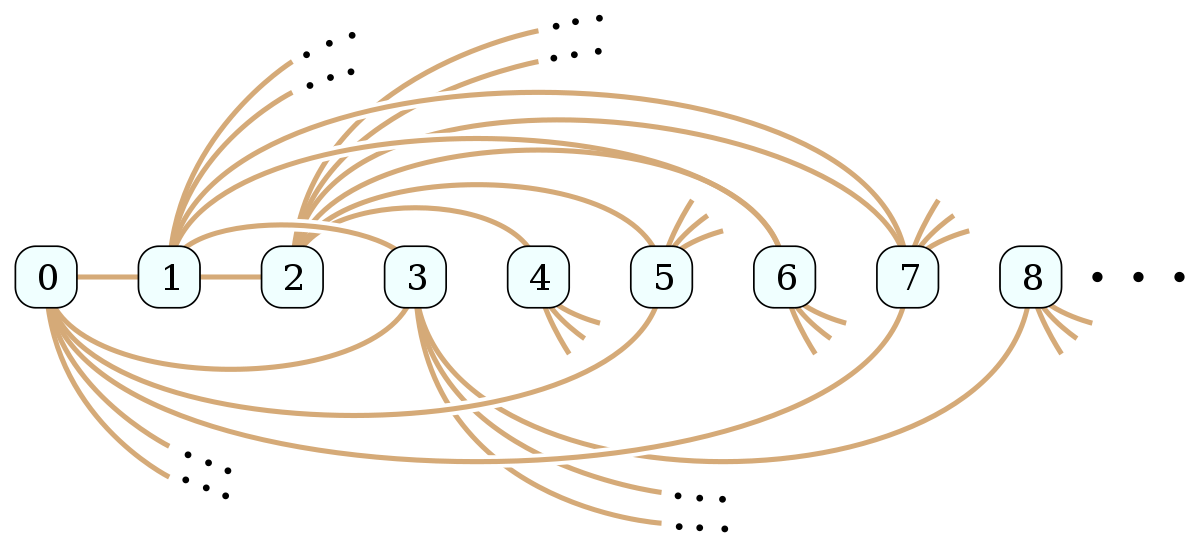
\includegraphics[scale=0.11]{figures/rado_graph.png}}. Even more, we have the following result:

\begin{theorem}
The Radó graph embeds into the curve graph of a surface $S$ if and only if $S$ has infinite genus.
\end{theorem}


Given that our interest is to find a model the most "uniformly" defined possible, the \textbf{Erdös-Rényi} appear to be suitable for us. This model describe random finite graphs so we'll have to give asymptotic arguments. This model consists in considering $n$ vertices and then each of the possibles edges appear with probability $p$. 

\begin{defini}
We will denote by $\G(n,p)$ to the probability space formed by all the graphs of $n$ vertices and probability measure 
$$ \P(G\in \G(n,p)) = p^{k} (1-p)^{\binom{n}{2}-k} $$
where $k$ is the number of edges in $G$, the $\sigma$-algebra is given by the power set.
\end{defini}

\begin{theorem}
Let $\omega(n)$ be a function that tends to infinity arbitrarily slow as $n$ tends to infinity
\begin{itemize}
\item If $p\geq \frac{log(n)+ \omega(n)}{n}$ then 
$$\lim_{n \to \infty} \P(G \in \G(n,p) \text{ is connected}) = 1$$
\item If $p\leq \frac{log(n)- \omega(n)}{n}$ then
$$\lim_{n \to \infty} \P(G \in \G(n,p) \text{ is disconnected}) = 1$$
\end{itemize}
\end{theorem}

\begin{theorem}
Let $\epsilon>0$ be fixed, $\epsilon n^{-3/2} \leq p = p(n) \leq 1 - \epsilon n^{-3/2}$, let $k = k(n)$ be a natural number and set $\lambda_{k} = \lambda_{k}(n) = n\cdot b(k;n - 1,p)$. Then the following assertions hold.

\begin{itemize}
\item If $\lim \lambda_{k}(n) = 0$, then $\lim P(X_{k} = 0) = 1$. 
\item If $\lim \lambda_{k}(n) = \infty$, then $\lim P(X_{k} > t) = 1$
for every fixed $t$.
\item If $0 < \lim\lambda_{k}(n) < \lim \lambda_{k}(n) < \infty$,
then $X_{k}$ has asymptotically Poisson distribution with mean $\lambda_{k}$: 
$$P(X_{k} = r) \sim e^{\lambda_{k}}\cdot \lambda_{k}^{r}/ r!$$
for every fixed $r$.
\end{itemize}
\end{theorem}
\begin{theorem}
Let $r = r(n) = O(n^{1/3})$ and let $p=p(n)$, $0<p<1$, be such that
$$\binom{n}{r} p^{\binom{r}{2}} \to \infty \text{ and } \binom{n}{r+1} p^{\binom{r+1}{2}} \to 0 $$
Then a.e $G_{p}$ has clique number $r$
\end{theorem}
\begin{theorem}
Let $c$ be a positive constant, $d=d(n)\geq 2$ a natural number, and define $p=p(n,c,d), 0<p<1$, by
$$p = \frac{\big( n\cdot log(n^2/c)\big) ^{1/d}}{n}$$
Suppose that $pn/(log\text{ }n)^{3} \to \infty$. Then in $G(n,p)$ we have
$$\lim_{n\to \infty} \P (diam\text{ }G = d) = e^{-c/2} \text{ and }  \lim_{n\to \infty} \P (diam\text{ }G = d+1) = 1 - e^{-c/2}$$
\end{theorem}

%------------------------------------------------------------------------
\noindent\hrulefill

{\Large \noindent \textbf{Rigidity}}

As we already mention, the importance of rigidity in mathematics is that it's a concepts that allows us to study the objects through the morphisms between them. In this context we have the celebrated result due to Ivanov which asserts that every automorphism of $C(S)$ is induced by a self-homeomorphism of $S$. A lot of work has been developed trying to generalize this result, in [J. Hernández]\cite{rigidExpJH} we can find a summary of the state of the art of this pipeline with the appropriate bibliographic references. 

There's a method to expand subgraphs developed in [Aramayona, Leininger]\cite{rigidExpJH} which can be used to obtain new results concerning edge-preserving maps. We took particular interest to this method due to it's combinatorial nature.

\begin{defini}
Let $\Gamma$ be a simplicial graph and let $H<\Gamma$ be a vertex-induced subgraph. A function $f:y\to \Gamma$ is \textbf{locally injective} if $f|_{star(v)}$\footnote{The $star(v)$ is the vertex-induced subgraph with vertices $\{ v \} \cup N(v)$ ($v$ plus its neighborhood).} is injective for all $v \in V(y)$. 
\end{defini}

\begin{defini}
$H<\Gamma$ is \textbf{rigid} if every locally injective function defined in $H$ can be extended to an automorphism of $\Gamma$. \end{defini}

A vertex $v \in V$ in a graph it's called to be uniquely determined by $A\subset V(G)$, denoted $v=<A>$, if $v$ is the unique neighbor of every element of $B$, i.e.

$$ \{ v \} = \bigcap_{w\in B} lnk(w) $$

\begin{defini}
The first rigid expansion of $Y\subset \Gamma$ is the vertex-induced subgraph whose vertices are
$$ V(Y) \cup \{ v\in V(\Gamma) :  \exists A \subset V(Y) \text{ where } v = <A>  \}$$
\end{defini}

In the probabilistic context we have the following calculations to study rigidity phenomena.

\begin{itemize}
\item What is the probability that a vertex $v$ is uniquely determined by a set of size $k$? (Event $E_1$)
 \item What is the probability that a set of size $k$ generate a rigid expansion? (Event $E_3$)
\end{itemize}

For the first event take a look to the following picture

\begin{figure}[h!]
	\centering
	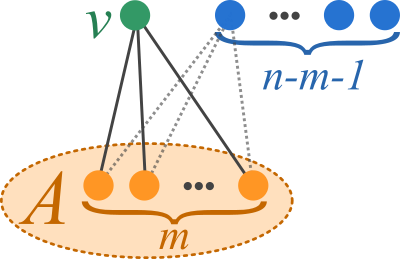
\includegraphics[scale=0.8]{figures/uni.png}
	\caption{Probability of uniquely determined vertices}
\end{figure}

i.e. if $<A> = v$ with $|A| = m$ then there's a edge between $v$ and every vertex in $A$, and none of the $n-m-1$ remaining vertices is also connected to every vertex in $A$, i.e.
$$\P(E_1(m)) = p^{m}(1-p^{m})^{n-m-1}$$

For the second question we have that if $A_k$ does not generate a rigid expansion is because none of the possible subsets of $A_k$ determined uniquely a vertex outside of $A_k$. 

We have that the probability that none of the vertices outside of $A_k$ is uniquely determined by $A_m\subset A_k$ is $\rho_{m,k} = (1 -  \P(E_1(m) )^{n-k}$.

$$\P(A_k \text{generates a rigid expansion}) = 1 -  \Pi_{m=1}^{k} (\rho_{k,m})^{\binom{k}{m}}  $$

Using the networkx library in python we obtained simulations for this phenomena and then compare them with the past calculations

\begin{figure}[h!]
	\centering
	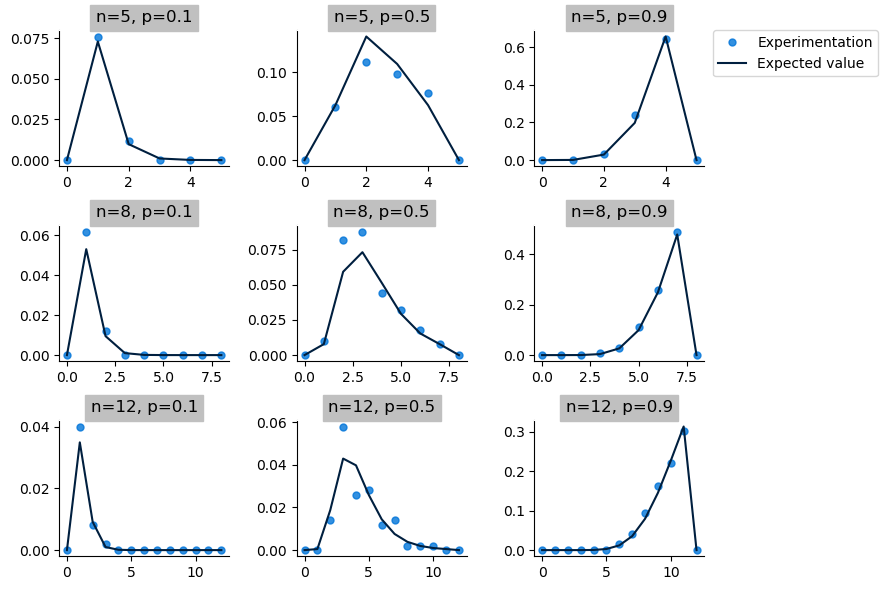
\includegraphics[scale=0.5]{figures/fixed-uniq-det.png}
	\caption{Probability of uniquely determined vertex, varying $k$ in $A_k$}
\end{figure}

\begin{figure}[h!]
	\centering
	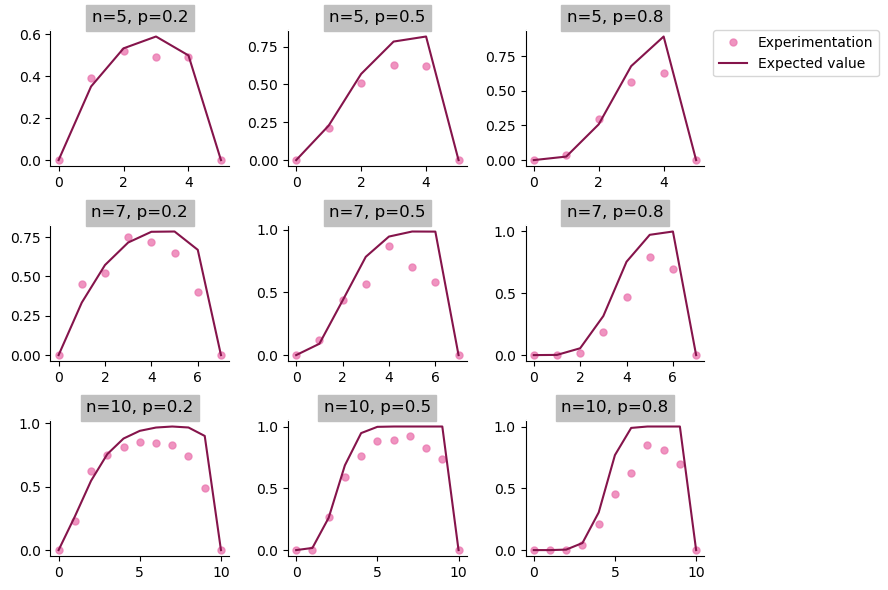
\includegraphics[scale=0.5]{figures/rig-prob.png}
	\caption{Probability of having a rigid expansion,  varying $k$ in $A_k$}
\end{figure}
%\newpage
\bibliographystyle{plain}
\bibliography{lab_notes}

\end{document}